\pdfminorversion=4
\documentclass[12pt]{tufte-book}
\usepackage[sfdefault]{roboto}
\usepackage[T1]{fontenc}
\usepackage{graphicx}
\usepackage{amsmath,amssymb}
\usepackage{natbib}
\bibliographystyle{chicago}
\usepackage{tikz}
\usetikzlibrary{positioning,calc,shapes,decorations.pathreplacing,shapes}
\usepackage{hyperref}
\usepackage{float} % allows figure inside minipage
% \usepackage[xindy,toc]{glossaries}
%\usepackage{natbib}
%\makeglossaries
\setcounter{secnumdepth}{2}
\newcounter{parnum}
\newcommand{\N}{%
  \noindent\refstepcounter{parnum}%
  \makebox[\parindent][l]{\textbf{\arabic{parnum}.}}}
\setlength{\parindent}{160em}

% Use a generous paragraph indent so numbers can be fit inside the
% indentation space.
% chapter format
\titleformat{\chapter}%
  {\huge\rmfamily\color{black}}% format applied to label+text
  {\llap{\colorbox{gray}{\parbox{1.5cm}{\hfill\itshape\huge\color{white}\thechapter}}}}% label
  {2pt}% horizontal separation between label and title body
  {}% before the title body
  []% after the title body

% section format
\titleformat{\section}%
  {\normalfont\Large\itshape\color{black}}% format applied to label+text
  {\llap{\colorbox{gray}{\parbox{1.5cm}{\hfill\color{white}\thesection}}}}% label
  {1em}% horizontal separation between label and title body
  {}% before the title body
  []% after the title body

% subsection format
\titleformat{\subsection}%
  {\normalfont\large\itshape\color{black}}% format applied to label+text
  {\llap{\colorbox{gray}{\parbox{1.5cm}{\hfill\color{white}\thesubsection}}}}% label
  {1em}% horizontal separation between label and title body
  {}% before the title body
  []% after the title body

\makeatletter
\renewcommand{\@tufte@reset@par}{%
  \setlength{\RaggedRightParindent}{1.0pc}%
  \setlength{\JustifyingParindent}{1.0pc}%
  \setlength{\parindent}{1pc}%
  \setlength{\parskip}{10pt}%
}
\@tufte@reset@par% chktex 1
\makeatother

% Needed for tikz flowchart
\pgfdeclarelayer{background}
\pgfdeclarelayer{foreground}
\pgfsetlayers{background,main,foreground}

\tikzstyle{datablock}=[draw, fill=blue!20, text width=5em,
    text centered, minimum height=2.5em]
\tikzstyle{ann} = [above, text width=5em]
\tikzstyle{modelfits} = [datablock, text width=6em, fill=red!20,
    minimum height=12em, rounded corners]
\def\blockdist{3.3}
\def\edgedist{3.5}
% end Needed for tikz flowchart

\title{MENE survey: Small Area Estimates}

\hyphenation{Map-Node}

%\author{City Science Corporation}

\renewcommand{\maketitlepage}{%
\tikz[remember picture,overlay] \node[opacity=1,inner sep=0pt] at
(current page.center){\includegraphics[width=\paperwidth,height=\paperheight]{corporate_images/bluebell}};

\vspace*{0.7\textheight}
\begin{figure}
\begin{center}
\begin{tikzpicture}[scale=2, transform canvas={scale=2}]
  \node[draw, fill=black, fill opacity=0.7, text=black, text opacity = 1,
        rectangle split, rectangle split parts=2, line width=0,
        align=center] (a) {
\Large{\color{green} Natural England}\\
\large{\color{white}\textit{Small Area Estimation feasibility: MENE survey}}
\nodepart{second}
\includegraphics[width=0.5\textwidth, trim=25pt 25pt 25pt 25pt]{corporate_images/csclogo.png}
};
\draw[ultra thick] (a.text split west) -- (a.text split east);
\end{tikzpicture}
\end{center}
\end{figure}

\thispagestyle{empty}%

}

\newcommand*{\blt}{
   \item[] \includegraphics[width=8pt]{corporate_images/cscbullet.png}
}



%\documentclass[a4paper,portrait,12pt]{article}
%\usepackage[latin1]{inputenc}
%\usepackage{setspace}
%\usepackage{graphicx}
%\usepackage{color}
%\usepackage{hyperref}
 
%\begin{document}
%\SweaveOpts{concordance=TRUE}

\begin{document}
\maketitle

\newpage
\begin{tabular}{ll}
{\color{blue}Date issued:} &  {\color{blue}15th May 2019}\\
{\color{blue}Document status:} & {\color{blue}Released}\\
{\color{blue}Version number:} & {\color{blue} 1.0}\\
{\color{blue}Document history:} & \\
\end{tabular}


\begin{tabular}{|l|l|l|}
\hline
Author & Version & Change Report \\
\hline
Paul Hewson & 0.1 & Initial templating\\
\hline
Paul Hewson & 0.2 & Add EDA \\
\hline
Paul Hewson & 0.3 & Add modelling \\
\hline
Paul Hewson & 0.4 & Add SAE \\
\hline
Paul Hewson & 0.5 & Release draft\\
\hline
Paul Hewson & 0.6 & Client revisions\\
\hline
Laurence Oakes-Ash & 1.0 & Release report\\
\hline

\end{tabular}                    

                    
{\color{blue}Prepared by:}
\begin{itemize}
\item[] Paul Hewson PhD CStat CSci
\end{itemize}

{\color{blue}Approved by:}
\begin{itemize}
\item[] Laurence Oakes-Ash BSc ACMA CGMA MCIHT Director
\end{itemize}

\newpage

\chapter{Project Aims}


\section{Overview}


\N Using data collected by the \emph{Monitor of Engagement with the Natural Environment (MENE survey)}, this project aims to determine whether Small Area Estimation (SAE) techniques can be used by Natural England to improve upon the accuracy and precision of survey-based estimates of the extent to which local populations engage with the natural environment. More specifically, it is concerned with quantifying improvements in accuracy and precision and determining what savings (in terms of effective sample sizes) can be achieved when applying SAE techniques at Local Authority level as well as illustrating the potential for use at the Middle Layer Census Super Output Area (MSOA).


\N Specifically for this evaluation, the request was to model responses to ``Q1: Volume of visits per day over last 7 days'' and ``Q17: Frequency of visits during last 12 months''.   Whilst an interesting range of attitudinal and other questions are asked which may be associated with these responses, in order to conduct small area estimation we have to match predictor variables which ones which can be found in some auxiliary data.   The variables identified as being of potential interest were:

\begin{itemize}
\item Age
\item Sex
\item Ethnicity
\item Marital status
\item Working status
\item Socio-economic group
\item Lifestage
\item Household size
\item Children in household
\item Adults in household
\item Tenure
\end{itemize}

It is also possible to use the geographical information provided.

\section{MENE survey data}

\N As currently available to us, the MENE survey comprises 420,790 responses. These have been accumulated over \emph{nine} years of the survey.

\begin{table}
\begin{tabular}{lr}
Dates & Responses \\
March 2009 - February 2010 & 48,514\\
March 2010 - February 2011 & 46,099\\
March 2011 - February 2012 & 47,418\\
March 2012 - February 2013 & 46,749\\
March 2013 - February 2014 & 46,785\\
March 2014 - February 2015 & 45,225\\
March 2015 - February 2016 & 45,965\\ 
March 2016 - February 2017 & 46,558\\
March 2017 - February 2018 & 47,477
\end{tabular}
\caption{Number of responses in the MENE survey data by year of survey}
\end{table}

\input{EDA.tex}
\input{Modelling.tex}


\chapter{Summary of Method}

\section{Small area estimation}
\label{sae_description}

\N Small Area Estimation (SAE) techniques have gained increasing acceptance over the last 3 decades\footnote{Rao, J.N.K. (2003) Small Area Estimation New York, Wiley}. There are a variety of well established approaches, the ones used here draw from model-based survey analysis and seek to ``pool'' evidence drawn from across a wider sample in order to ``enhance'' local estimates\footnote{Gelman, A. and Hill, J. (2007) Data Analysis Using Regression and Multilevel/Hierarchical Models Cambridge, CUP}.   They are considered to have some similarities with a post-stratification based approach in design based survey methods.


\N The core idea of this approach to small area estimation is set out in figure~\ref{sae_pic}.


\begin{figure}
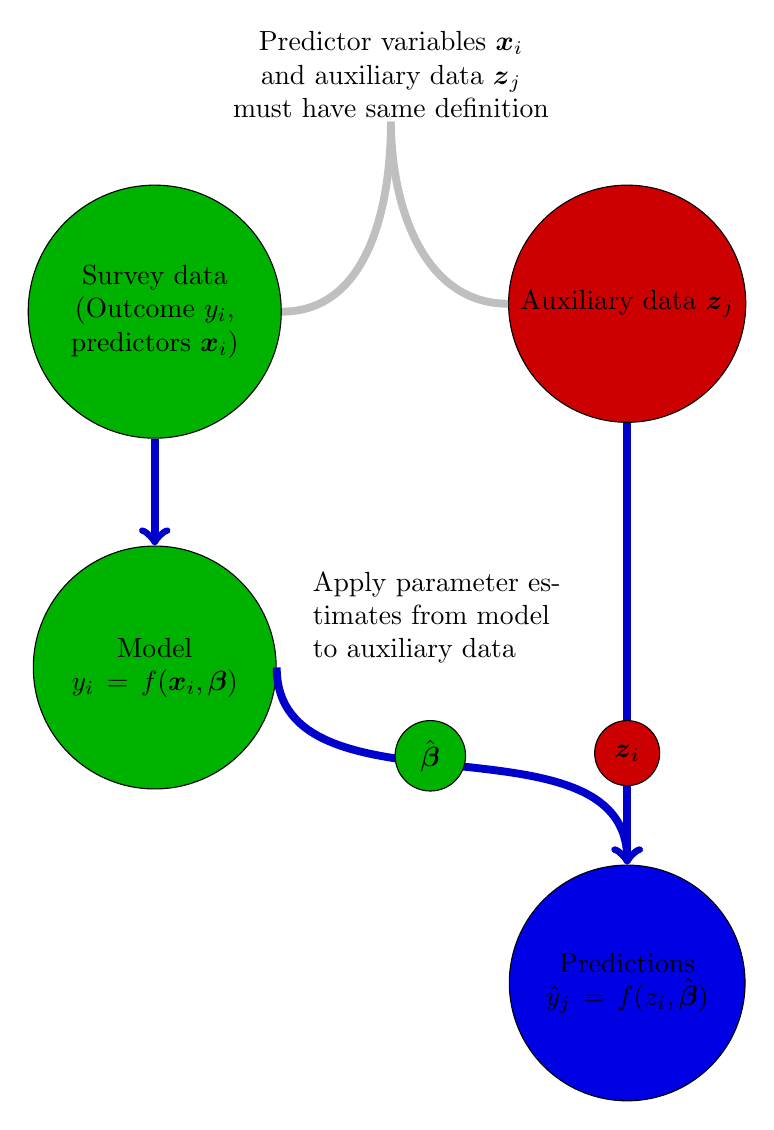
\begin{tikzpicture}[%
  % common options for blocks:
  block/.style = {draw, fill=blue!80!black, align=center, anchor=west,
              minimum height=0.65cm, inner sep=0},
  % common options for the circles:
  ball/.style = {circle, draw, align=center, anchor=north, inner sep=0}]
% Data sources
\node[ball,text width=3cm,fill=green!70!black] (survey) at (6,0) {Survey data (Outcome $y_i$, predictors $\boldsymbol{x}_i$)};
\node[ball,text width=3cm,fill=red!80!black] (aux) at (12,0) {Auxiliary data $\boldsymbol{z}_j$};

\node[anchor=north,text width=5cm,inner sep=.05cm,align=center,fill=white]
  (match) at (9,2) {Predictor variables $\boldsymbol{x}_i$ and auxiliary data $\boldsymbol{z}_j$ must have same definition};
\draw[-,line width=1mm,draw=gray!50] (survey.east) to [out=360,in=270] (match.south);
\draw[-,line width=1mm,draw=gray!50] (aux.west) to [out=180,in=270] (match.south);


\node[ball,fill=green!70!black,text width=3cm,anchor=base] (model) at (6,-6) {Model $y_i=f(\boldsymbol{x}_i, \boldsymbol{\beta})$};
\node[ball,fill=blue!90!black,text width=2.9cm,anchor=base] (preds) at (12,-10) {Predictions $\hat{y}_j = f(z_i, \hat{\boldsymbol{\beta}}$)};

% arrows showing split from all women to cancer and ~cancer
\draw[->,line width=1mm,draw=blue!80!black] (survey.south) to [out=270,in=90] (model.north);
\draw[->,line width=1mm,draw=blue!80!black] (model.east) to [out=270,in=90] (preds.north);
\draw[->,line width=1mm,draw=blue!80!black] (aux.south) to [out=270,in=90] (preds.north);


% transition from all women to actual cancer rates

% note illustration the p{cancer} circle (text won't fit inside)
\node[inner sep=0,anchor=west,text width=3.3cm] (note1) at (8,-5.5) {
   Apply parameter estimates from model to auxiliary data};
\node[ball,text width=.8cm,fill=green!70!black] (betahat) at (9.5,-6.8) {
   $\hat{\boldsymbol{\beta}}$};
\node[ball,text width=.8cm,fill=red!80!black] (z) at (12,-6.8) {
   $\boldsymbol{z}_i$};
\end{tikzpicture}
\label{sae_pic}
\caption{Basic outline of synthetic small area prediction}
\end{figure}



\noindent There are similarities to post-stratification (a very well established design based approach to survey estimation)\footnote{Andrew Gelman and Thomas C. Little (1997), ``Poststratification Into Many Categories Using Hierarchical Logistic Regression'', Technical report, University of Columbia}.   The advantages of a modelling based approach (Bayesian or otherwise) are the way additional multilevel data can be structured.  Auxiliary data can be taken from a variety of sources including the relative spatial structure of the sampling points. An advantage of Bayesian methods are that provided the variables used for conventional weighting are used in fitting the models, this account for the sampling pattern.


\N Focusing on the behaviour of individual respondents nested within local authorities -- a classic ``multilevel'' scenario -- this study has adopted a conventional approach to dealing with hierarchically structured data with a simple count response; namely generalized linear mixed-effects regression modelling. It is an approach that aims to capture, as far as possible, the relationship between the response (or dependent variable) and a number of independent variables which include categorical variables describing individuals' tenure, age, sex, ethnicity, disability, marital status, work status, social classification, lifestage, adults / children in household, size of household, working status, car ownership and their self reported general health\footnote{In order to achieve some parsimony, different models draw upon different sets of categorical variables, for example age may be split into different bands.} The multilevel models are thus used to estimate individual level parameters that explain the relationship between these categorical variables and the response, whilst simultaneously allowing for a random intercept that is unique for each local authority and which describes any systematic authority-by-authority variation in the response that is not explained by the individual-level model.


\N Thus for each individual $i$ in area $j$, the outcome reports the number of trips made to the natural environment in either the last week or the last year We model this as a Poisson distributed random variable so that:

\begin{equation}
Y_{ij} \sim Bernoulli(p_{ij})
\end{equation}


where the propensity that individual $i$ has reported a given number of trips is given by:

\begin{equation}
  logit(p_{ij}) = \boldsymbol{x}_{ij}^T \boldsymbol{\beta}
\end{equation}


where $\boldsymbol{\beta}$ denotes the model parameters and $\boldsymbol{x}$ denote individual characteristics recorded in the survey (such as age, gender, etc.) classified as categorical variables.


\N Throughout this report we have assumed that the intercept term varies by local authority, but with the constraint that all these random intercepts are drawn from a common Normal distribution with zero mean and unknown variance.   We further extend this model to allow the local authority random intercepts themselves to have a linear predictor.  This could be used to capture contextual information that varies by residence rather than by individual. If this were to be undertaken the intercept for Local Authority $j$ would be given as: $\boldsymbol{z}_{j}^T \boldsymbol{\zeta}$ where $\boldsymbol{\zeta}$ denote the upper-level parameters and $\boldsymbol{z}$ denote area-level characteristics which describe various aspects of the local authority as a whole.  The linear predictors could be further nested to include, for instance, a term for smaller areas (such as MSOAs) within the local authority.


\N Conventional (i.e. frequentist) approaches were employed for model exploration, but for the final model fit (used to generate the Local Authority estimates) a Bayesian approach was adopted. At this stage each of the ``fixed effects'' (the parameters relating various factors to the response) were drawn from a Normal distribution with a prior mean of zero and diffuse variance of 0.001.  The variance term for the random interceptwas assumed to be Uniform (0, 100).   These models have been fitted in R using the STAN software package\footnote{Stan Development Team (2018). RStan: the R interface to Stan. R package
  version 2.18.2. http://mc-stan.org/.}.


\N Having obtained estimates of the individual level parameters, it is possible to apply these to the ``known'' population structure of a given local authority to produce an estimate of the statistic of interest. This would, in effect, represent the expected response for that local authority given its specific socio-demographic composition. However, the strength of multilevel modelling is that, by estimating individual level effects for typical respondents of each type, the data is used to estimate how responses in each local authority differ from the expected national response. The resulting local authority ``random effects'' are then used, along with the individual level responses, to make ``small area predictions'' of the statistic of interest in each local authority. 


\N By taking a modelling approach it is also possible to eliminate ``nuisance parameters''. For example, the trend over time for the years that the survey has been running is obviously of interest in its own right, but is not relevant to attempting to make small area predictions in the same time frame as the most recent data. Consequently, time can be regarded as a nuisance variable, and conditioned out of the model so that all years data can be used to esimate the relationship between predictors and the number of trips made.


\N The Small Area Estimation approach requires that the number of people in each LA with each unique combination of characteristics used in the model is known, or can be estimated. Thus for the engagement models used it is necessary to know how many people are aged 16-24, own a car, are employed, owner occupiers and have a professional occupation -- and how many people there are with every other possible combination of characteristics used in the model . This data is obtained by taking the detailed socio-economic composition of Local Authorities from the 2011 Census Small Area Microdata (SAM) 5\% Sample, and constraining that distribution to mid-2016 age-sex population totals.  

\section{Precision and accuracy}

\N Our concern with \textsf{precision} refers to the level of certainty which the various methods attach to their estimates of self-reported engagment with the natural environment. These are conventionally understood with reference to the 95\% Confidence Intervals (CIs) associated with the various estimates. More precise measures will have narrower 95\% CIs, and any improvement in precision can be measured by comparing the width of SAE-based \textsf{modelled} estimate 95\% CIs with the original sample-based \textsf{direct} estimate 95\% CIs. Our \textsf{specific} goal here is to express the impact of SAE-based modelling in terms of 'effective sample sizes' and thus predict how much smaller the \emph{MENE survey} samples would need to be in order to achieve the precision achieved by design based survey methods.


\N The measurement of \textsf{accuracy} is less straightforward in that we do not know with any certainty the \textsf{actual} number of people engaging with the natural environment in each Local Authority. There are thus no definitive ``correct'' values against which to compare the direct and modelled estimates produced using \emph{MENE survey} data. 




\section{Engagement and LA-Level Estimates}


\N Local Authority random effects, are obviously to be included in the model used to estimate rates of physical activity. These parameters, one for each local authority covered by the analysis effectively measure the extent to which responses in each area differ from what might be expected given the individual level (fixed effects) logistic regression model. These LA-specific intercepts effectively describe how much up or down the fixed effects logistic regression curve must move to best fit the observed data for each local authority.


\N Few of the LA-level fixed effects would be regarded as statistically significant at the 95\% level in a conventional analysis.   However, this is a mechanism for capturing uncertainty in the modelled responses, and has the effect of reducing the level of uncertainty and hence increasing the precision of many estimates.   It would be possible to use better models, such as allowing the random effects to be spatially correlated. This may in turn increase the precision of the subsequent small area estimates.


\N Having obtained ``fixed'' and local authority ``random effect'' parameter estimates, these can applied to socio-demographic data for Local Authorities and subsequently, by IPF, to MSOAs. These, as discussed above, are derived from 2011 Census Small Area Microdata, constrained to mid-2016 ONS age-sex totals in local authorities and MSOAs. Thus having determined how many people in each local authority are in each unique 'person-type' cell defined by the model, and having multiplied those sub-populations by the likelihood that those person-types will take a trip to the natural environment, the resulting counts are summed to obtain estimates of the overall number of people in each local authority who took a trip.



\N As already intimated, by modelling the relationship between a range of independent covariates and the dependent variable (in this case whether or not individuals have made a trip in the last week/year) allowance is automatically made for any unintended and unknown bias in the sample. For instance, it is very unlikely that whether or not an individual has a self reported health status of ``bad'' will ever be used as either a sampling or weighting factor. Yet it is quite likely that among a large number of relatively small sub-samples (which, in this case, are the local authority subsets of the \textsf{MENE survey} there will be a number instances in which a particular sample is very unrepresentative of its underlying population. Given that general health has, as illustrated in , a strong (and of course entirely expected) impact on engagement with the environment, this inevitably means that at least some of the sub-samples will return biased sample-based direct estimates of local levels of physical activity.

\input{SAE.tex}

\input{SAE_forecasts.tex}


\chapter{Conclusions}

\section{Synthetic small area estimates}

\N The synthetic small area estimates for the two outcome variables (Q1 and Q17) are made available as a set of \texttt{.csv} files giving the ONS code for the small area (Local Authority and MSOA) along the posterior median and 95\% credible intervals for the estimated number of people who made a trip in the last week, or who made a trip more than once of twice in the last year.   The R code necessary to reproduce this analysis is available in a github repository.

\N This feasibility study has demonstrated the viability of a small area approach to the MENE survey.   Tables~\ref{q1_rms} and \ref{q17_rms} indicate a constructed Residual Mean Square Error (RMS) estimate to illustrate the likely effect of reducing sample size.   It can be seen that sample size reductions have less impact in terms of Q1 (trips in the previous week) than Q17 (at least monthly trips in previous year).   There are two points to note. Firstly, the RMS is computed using the entire dataset for 2015/16 as the ``gold standard''. Clearly, it would be preferable to have an actual ``gold standard''; most methodological studies in small area estimation conduct an entirely simulation based exercise where the entire population is synthesised, a sample taken and the small area estimates compared the the simulated ``gold standard'' or ``ground truth''.  Therefore these RMS estimates can not be used to compare this method with any other; they can only be used internally, to demonstrate how the quality of the estimates decreases with sample size.

\N It is apparent from several of the caterpillar plots presented that, when using data from 2015/16, the interval estimates for several local authorities are extremely wide.  This is because there were few or no respondents from those local authorities in that year.   There are two solutions to this problem.  The first is to establish an upper level model for the survey geography. Allowing spatially correlated random effects would mean that the random effect for any local authority would be based on its neighbours values as well as its own.   A more data driven approach would be to develop an upper level model based on local authority specific predictor variables.    We would further recommend for any subsequent small area estimation that all available years' data should be used, which would allow a data driven model to use patterns between individuals and areas to be established, even allowing for changes over time.

\N There are some data challenges to be reconciled. Firstly, ownership of a car is a strong predictor of engagement with the natural environment, yet does not seem to be recorded in the most recent two years of the available survey.   This reduces the precision by which small area estimation methods can predict a response.  We would recommend that this question be restored in subsequent years.  It is possible to incorporate missing data imputation methods within a Bayesian framework and this could be done in a definitive study and data from 2016/17 and 2017/2018 could be used to get stronger evidence on the relationship between other person type variables and geographical information. However, whilst Bayesian methods are powerful, they are not a magic wand and data would always be preferred to any compensatory technique.

\N There are other questions (general health) which are also only avaialble for certain years.   More significantly, there are other survey questions which have drifted from the census definitions; for example limiting long term illness in the census now records at three levels but the MENE survey has a simple yes/no question in response to disability. Small area estimation, and many techniques around non-random sampling which aim to weight a sample after the event (e.g. post-stratification) require that auxiliary variables are available which match the variables in the survey of interest.   It is always a balance between maintaining a consistent data collection over time and keeping up to date with external changes.  However, we would suggest that a modelling based approach allows any changes to be modelled and hence the advantages seem to lie more with consistency between the MENE survey and external data. If the MENE survey were ever to be based on a non-random sampling frame (such as happens in web-surveys) we would suggest that the need to match respondent information with auxiliary data becomes even more important.

\N It would seem that, using appropriate small area estimation methods, a reduction in sample size is possible.  The challenge in this work is that it assumes that the model is essentially correct.   It assumes that specific person types generally behave the same wherever they are in the country with the exception of an overall local effect captured by the local authority specific random effects.  This is rarely a popular assumption with local authorities being judged on the output of such a modelling exercise.  It is possible with more judicious modelling (such as spatial random effects models using the postcode sector of the respondent) to better estimate local authority specific random effects. Clearly this requires both further technical work and further discussions with stakeholders as to the likely acceptablility of such modelling.   Similarly, producing more granular geographical results such as MSOA level small area estimates, while feasible perhaps merits further work looking at local specific effects.

\N It is possible to produce small area estimates for finer domains, such as MSOAs. These results are given in a csv file.  These may be useful in terms of identifying groups of people who are not making the most of contact with the natural environment. We would however suggest that this does not necessarily require small area estimates, but that the same understanding could be gained by carefully examining the model results. For example, the ``fixed effects'' provide information on types of people who have differential access to a natural environment.   Local authority random effects provide information on areas of the country where access might be higher or lower than the average, assuming every part of the country had the same mix of people types.

\chapter{Appendix}

\section{Technical clarifications}

\subsection{Odds and odds ratios}


\fbox{
\begin{minipage}[t]{0.9\textwidth}
The proportion is a well recognised summary metric:
  
\begin{displaymath}
Proportion = \frac{\mbox{Number of individuals responding with `yes'}}{
      \mbox{Total number of individuals surveyed}}
\end{displaymath}

In many fields (including medicine) it is common to use odds as a
summary metric:

\begin{displaymath}
Odds = \frac{\mbox{Number of individuals responding with `yes'}}{
    \mbox{Number of individuals responding with `no'}}
\end{displaymath}
\end{minipage}
}


The odds ratio is a less commonly used summary measure of treatment /
exposure effect.   It is defined as:

\fbox{
\begin{minipage}[t]{0.9\textwidth}
\begin{displaymath}
Odds\ ratio = \frac{\mbox{Odds of `yes' for group A}}{
  \mbox{Odds of `yes' for group B}}
\end{displaymath}
\end{minipage}
}

An odds ratio with value of (almost) 0 indicates that the
odds of replying `yes' for group `A' are either very low (almost zero
respondents replied `yes') or the odds of replying `yes' for group `B' are
very high (almost every respondent replied `yes') or both.   An odds ratio of 1
indicates that the odds of replying `yes' are the same in both groups,
regardless of the relative number in each group who replied `yes'.   Odds ratios
above 1 indicate that relatively more respondents in group `A' replied yes
than did respondents in group `B'.

The log-odds ratio is the (natural) logarithm of the odds ratio.

\fbox{
  \begin{minipage}[t]{0.9\textwidth}
\begin{displaymath}
 Log Odds\ ratio = \log_e \left( \frac{\mbox{Odds of `yes' for group A}}{
     \mbox{Odds of `yes' for group B}} \right)
\end{displaymath}
\end{minipage}
}

The effect of using a log-odds ratio might be for visual or interpretative
reasons.   An odds ratio of 0.5 and an odds ratio of 2 indicate that the odds
of replying `yes' in group `A' are either half of twice the odds of group `B'.
There is a symmetry here which cannot be seen if these effects were to be
plotted.   Another reason, is that standard modelling approaches naturally
work with the log-odds ratio for their own reasons.

  
\fbox{
\begin{minipage}[t]{0.9\textwidth}
  As a point of clarification for later, it is possible to convert a proportion
  into an odds using formula~\ref{odds_prop}

\begin{equation}
Odds = \frac{Proportion}{1-Proportion}
\label{odds_prop}
\end{equation}
\end{minipage}
}



\subsection{Logistic regression models}

This analysis considers two dichotomous outputs, namely whether a respondent
indicated that they have made at least one trip in the last week, or whether
over the course of the previous year they had made more than one trip a
month.   Denoting the number of individuals by $n$, and a single
individual with a subscript $i$ (where $i = 1, \ldots, n$).
for individual $i$, the response variables are created as:

\textbf{Question 1}


\begin{displaymath}
Y_i = \left\{ \begin{array}{rll}
1 & \mbox{ if } &\mbox{ if one or more trips have been made in the last week}\\
0 & & \mbox{otherwise}
\end{array} \right.
\end{displaymath}

\textbf{Question 17}


\begin{displaymath}
Y_i = \left\{ \begin{array}{rll}
             1 & \mbox{ if } &\mbox{ if trips have been made more than
                                     once a month in the last year}\\
0 & & \mbox{otherwise}
\end{array} \right.
\end{displaymath}


For technical reasons, the standard statistical method for fitting a model to
such data is the so-called logistic regression.   There are three elements
to these models.

\begin{enumerate}
\item Assume that the response variable $Y_i$ is a realisation of a
  Bernoulli random variable where the probability $Y=1$ is given by $\theta_i$.
\item Next assume that there it is resonable to relate the outcome
  to a standard linear predictor of the
  form $\eta_i = \beta_0 + \beta_1 x_{i1} + \ldots + \beta_p x_{ip}$ where
  $\beta_j$ (with the subscript $j=1, \ldots, p$ denoting a distinct predictor
  variable from $1$ to $p$) are the parameters to be estimated and
  $\boldsymbol{x_i}=(x_{i1}, \ldots, x_{ip})$ are the values of the predictor
  variables for individual $i$.
\item In many ways, the $\eta_i$ values are similar to the $\hat{y}$ values
  of a standard linear regression.  However, we need a way of mapping these
  linear predictor values onto the probability $\theta_i$ that individual $i$
  reported having taken trip in the last week, or a trip more than once a month
  in the last year.   To do this, a so-called logistic link function is used.
\end{enumerate}

\begin{equation}
\log \left( \frac{\theta_i}{1-\theta_i} \right) = \eta_i
\label{logit_link}
\end{equation}

Equation~\ref{logit_link} is referred to as the \emph{logistic link} function
and is the reason these models are referred to as ``logistic regression''
models. It is something of a default in medical research where they have been
used for over a century. In 1972 \cite{nelder1972generalized} developed a
flexible framework for a range of related models.   From the point of view
of someone wishing to interpret the parameter estimates from a logistic
regression model, it can be seen that there is a similarity between this
function and the formula given in equation~\ref{odds_prop}.   What this means
is that the entire linear predictor (and the intercept on its own) are
effectively the (natural) log odds of a respondent answering a question
with `yes'.   The other parameters are the (natural) log-odds ratio for a
'yes' response for a member of the group described by that predictor variable
relative to the baseline.   For example, the log-odds ratio of a male respondent relative to a female replying `yes' to the question about trips.


For reference purposes, the inverse function to the logistic
link~\ref{logit_link} is as follows:

\begin{displaymath}
\theta_i = \frac{\exp(\eta_i)}{1 + \exp(\eta_i)}
\end{displaymath}

In other words, we can use this to calculate the probability that a particular
respondent replied `yes' to the dichotomised trip question.




\bibliography{../doc/refs}

\end{document}
